\lab{GMRES}{GMRES}
\label{lab:GMRES}
\objective{In this lab we will learn how to use the GMRES algorithm.}

The GMRES ("Generalized Minimal Residuals") algorithm is an efficient way to solve large linear systems.
It is an iterative method that uses Krylov subspaces to reduce a high-dimensional problem to a sequence of smaller dimensional
problems.

\begin{comment}
\section*{The Arnoldi Iteration and Approximate Solutions}
The basic idea of GMRES is as follows.
Let $A$ be an $m\times m$ matrix (real or complex), where $m$ is very large,
and let $b \in \mathbb{F}^m$ ($\mathbb{F}$ may either be the real or complex numbers).
Let $\mathcal{K}_n$ denote the order-$n$ Krylov subspace generated by $A$ and $b$.
In each iteration, we consider the least squares problem
\begin{equation}
\underset{x \in \mathcal{K}_n}{\text{minimize}}\qquad \|b-Ax\|_2.
\label{eq:GMRES_lstsq1}
\end{equation}
Now if $x \in K_n$, then $x$ can be expressed as a linear combination of basis vectors $b, Ab, \ldots, A^{n-1}b$, i.e.
\[
x = y_1b + y_2Ab + \cdots + y_nA^{n-1}b.
\]
If we let $K_n$ be the matrix whose columns are $b, Ab, A^{2}b, \cdots, A^{n-1}b$, then we can write this simply as
$x = K_n y$.
Then the solution of the least squares problem is the vector $K_{n}y$ such that $\|b-A K_{n}y\|_2$ is minimized.
\begin{figure}
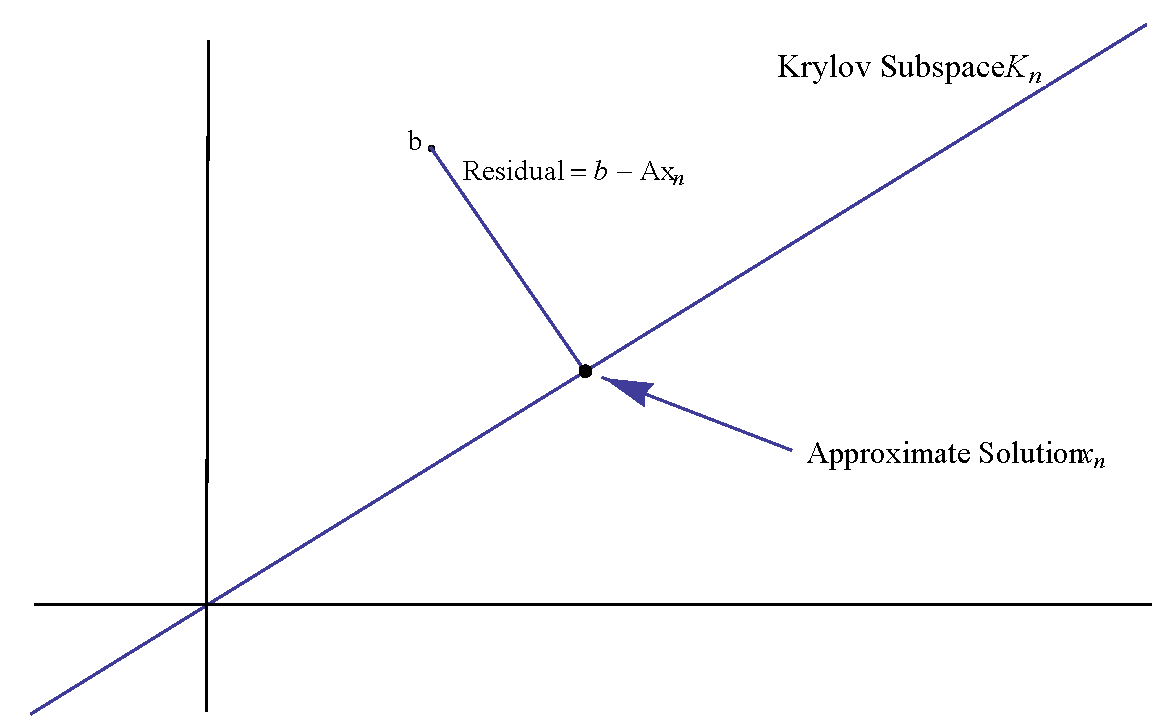
\includegraphics[width=\textwidth]{LeastSquares}
\caption{GMRES involves solving the least squares problem repeatedly.}
\end{figure}

The major drawback of this approach is that it relies on the matrix $K_n$, which tends to be ill-conditioned due to its columns
being far from orthogonal (as discussed in Lab \ref{lab:kry_arnoldi}).
%To see this, suppose there is an eigenbasis for $A$ with associated eigenvalues, and suppose $\lambda$ is the largest eigenvalue.
%Then $\lambda^n$ is an eigenvalue of $A^n$.
%Since $\lambda$ is bigger than the other eigenvalues of $A$, $\lambda^n$ may be much, much bigger than the other eigenvalues of $A^n$,
%which are simply the eigenvalues of $A$ raised to the $n$th power.
%Thus the eigenvector associated with $\lambda$ often begins to dominate as we progress, with the end result being that the columns of
%$K_n$ become nearly linearly dependent.
The easiest fix in this situation is to use the Arnoldi iteration so that we have an orthonormal basis for $\mathcal{K}_n$ to work with.
Not only does this alleviate the problem of ill-conditioning, it also allows us to optimize in other ways, due to the special
structure of the matrices produced.

Let $q_1,\ldots, q_n$ be the orthonormal basis for $\mathcal{K}_n$ obtained by the Arnoldi iteration, and let $Q_n$ be the matrix
having these vectors as its columns.
Recall that $q_1 = b/\|b\|_2$.
Finally, let $H_n$ be the $(n+1)\times n$ upper Hessenberg matrix generated by the Arnoldi iteration, and let $e_1=(1,0,\cdots,0)$.

In this orthonormal basis, $x \in \mathcal{K}_n$ implies that there is some vector $y$ such that $x = Q_n y$.
Further, it is not hard to check that the matrices generated by the Arnoldi iteration satisfy the equation
\[
AQ_n = Q_{n+1}H_n.
\]
We also have the identity
\[
b = \|b\|_2q_1 = \|b\|_2Q_{n+1}e_1.
\]
Putting all of this together, we can rewrite the objective function of our least squares problem as follows:
\begin{align*}
\|b - Ax\|_2 &= \|Ax - b\|_2\\
&= \|AQ_ny - b\|_2\\
&= \|Q_{n+1}H_ny - \left(\|b\|_2Q_{n+1}e_1\right)\|_2\\
&= \|Q_{n+1}\left(H_n y - \|b\|_2e_1\right)\|_2.
\end{align*}

The matrix $Q_{n+1}$ has orthonormal columns, but it does not have enough columns to be a unitary matrix.
Let us extend the set $q_1,\ldots, q_{n+1}$ to an orthonormal basis $q_1,\ldots,q_{n+1},q_{n+2},\ldots,q_m$
of our space, and let $Q'$ be the matrix whose columns are equal to these vectors.
Then $Q'$ is now a unitary matrix, and hence preserves the norm, i.e. $\|Q'z\|_2 = \|z\|_2$ for all $z \in \mathbb{F}^m$.
Given $x \in \mathbb{F}^{n+1}$, if we define $x' \in \mathbb{F}^m$ to be
\[
x' =
\begin{bmatrix}
  x\\
  0\\
  \vdots\\
  0
\end{bmatrix},
\]
then you can easily check that
\[
Q'x' = Q_{n+1}x.
\]
From this, we deduce that
\begin{align*}
\|Q_{n+1}x\|_2 &= \|Q'x'\|_2\\
& = \|x'\|_2\\
&= \|x\|_2.
\end{align*}
Hence, we conclude that
\[
\|Q_{n+1}\left(H_n y - \|b\|_2e_1\right)\|_2 = \|H_n y - \|b\|_2e_1\|_2.
\]
Thus, the least squares problem given by \ref{eq:GMRES_lstsq1} is equivalent to the problem
\begin{equation}
\underset{y \in \mathbb{F}^n}{\text{minimize}}\qquad \|H_n y - \|b\|_2e_1\|_2.
\label{eq:GMRES_lstsq2}
\end{equation}
If $y$ is the solution to this problem, then the solution to \ref{eq:GMRES_lstsq1}, and hence an approximate
solution to $Ax = b$ is given by $x=Q_n y$.

We can measure how good our approximate solution is by considering the residual, which we define to be
\[
\frac{\|Ax-b\|_2}{\|b\|_2}.
\]
We can express this residual in terms of $y$ as follows:
\begin{equation}
\frac{\|H_n y - \|b\|_2e_1\|_2}{\|b\|_2}.
\label{eq:GMRES_residual}
\end{equation}
\end{comment}

\section*{The GMRES Algorithm}
Let $A$ be an invertible $m \times m$ matrix and let $\b$ be an $m$-vector.
Let $\mathcal{K}_n(A, \b)$ be the order-$n$ Krylov subspace generated by $A$ and $\b$.
The idea of the GMRES algorithm is that instead of solving $A\x = \b$ directly, we use least squares to find $\x_n \in \mathcal{K}_n$ that minimizes the residual $r_n = \|\b - A\x_n\|_2$.
The algorithm returns when this residual is sufficiently small.
In good circumstances, this will happen when $n$ is still much less than $m$.

The GMRES algorithm is implemented with the Arnoldi iteration for numerical stability.  The Arnoldi iteration produces $H_n$, an $(n+1)\times n$ upper Hessenberg matrix; and $Q_n$, the matrix containing the basis vectors of $\mathcal{K}_n(A, \b)$.  Since the columns of $Q$ are orthonormal, and $AQ_n = Q_{n+1}H_n$, we can compute the residual equivalently as
\begin{equation}
\qquad \|\b - A\x_n\|_2 = \|H_n \y_n - \beta e_1\|_2.
\label{eq:GMRES_lstsq1}
\end{equation}

Here $\e_1$ is the vector $(1, 0, \ldots, 0)$ of length $n+1$.  $\beta$ is the Euclidean norm of $\b - A\x_0$, where $\x_0$ is an initial arbitrary guess of the solution.  (Ordinarily this guess is zero, and then the $A\x_0$ could be left out; however, a modified version of the algorithm will be discussed at the end of the lab, in which other nonzero guesses will be made.)  Thus to minimize the left side of \ref{eq:GMRES_lstsq1}, we can minimize the right, and $\x_n $ can be computed as $ Q_n \y_n + \x_0$.

This algorithm is outlined in Algorithm \ref{alg:gmres}.
For a complete derivation see [TODO: ref textbook].

\begin{comment}
so that instead of solving \eqref{eq:GMRES_lstsq1}, at the $n^{th}$ iteration we solve
\begin{equation}
\underset{\y \in \mathbb{F}^n}{\text{minimize}}\qquad \|H_n \y - \|\b\|_2\e_1\|_2.
\label{eq:GMRES_lstsq2}
\end{equation}
Here, $H_n$ is the $(n+1)\times n$ upper Hessenberg matrix generated by the Arnoldi iteration and $\e_1$ is the vector $(1, 0, \ldots, 0)$ of length $n+1$.
If $\y$ is the minimizer for the $n^{th}$ iteration of \eqref{eq:GMRES_lstsq2}, then the residual is
\begin{equation}
\frac{\|H_n \y - \|\b\|_2\e_1\|_2}{\|\b\|_2},
\label{eq:GMRES_residual}
\end{equation}
and the corresponding minimizer for \eqref{eq:GMRES_lstsq1} is $Q_n\y$, where $Q_n$ is the matrix whose columns are $\q_1, \ldots, \q_n$ as defined by the Arnoldi iteration.
This algorithm is outlined in Algorithm \ref{alg:gmres}.
For a complete derivation see [TODO: ref textbook].
\end{comment}

\begin{algorithm}
\begin{algorithmic}[1]
\Procedure{GMRES}{$A, \b, \x_0, k, tol$}
	\State $Q \gets \allocate{\size{\b}}{k+1}$			\Comment{Initialize}
	\State $H \gets \zeros{k+1}{ k}$
	\State $r_0 \gets \b - A\x_0$
	\State $Q[:,0] = r_0/\norm{r_0}_2$
    \For{$n=1\ldots k$}
        \State Set entries of $Q$ and $H$ as in Arnoldi iteration.
        \State Compute the residual $res$ and the least squares solution $\y_n$ for the part of $H$ so far created (equation \ref {eq:GMRES_lstsq1}).
        \If{$res < tol$}
            \State \pseudoli{return} $Q[:,:n+1]\y + \x_0, \,\, res$
        \EndIf
    \EndFor
    \State \pseudoli{return} $Q[:,:n+1]\y + \x_0, \,\, res$						
\EndProcedure
\end{algorithmic}
\caption{The GMRES algorithm. This algorithm operates on a vector $\b$ and matrix $A$. 
It iterates $k$ times or until the residual is less than $tol$, returning an approximate solution to $A\x=\b$ and the error in this approximation.}
\label{alg:gmres}
\end{algorithm}

%\begin{warn}
%The Python function \li{linalg.lstsq} solves a least squares problem, returning not only the vector, $y$, but also the residual,
%the rank of the matrix, and the singular values.
%Be careful when you write your code that you access the correct results and don't just assume that \li{linalg.lstsq} returns the
%vector that you want.
%The least squares solver also returns a residual, but it's not the number we reference in this book, so be sure to take the square
%root of the residual reported by the solver and divide by $\norm{b}$ to get $res=\norm{Ax-b}/\norm{b}$.
%\end{warn}
% Hint: explain how to find lstsq to find the residual?

\begin{problem}
Use Algorithm \ref{alg:gmres} to complete the following Python function implementing the GMRES algorithm.
\begin{lstlisting}
def gmres(A, b, x0, k=100, tol=1e-8):
    '''Calculate approximate solution of Ax=b using GMRES algorithm.
    
    INPUTS:
    A    - Callable function that calculates Ax for any input vector x.
    b    - A NumPy array of length m.
    x0   - An arbitrary initial guess.
    k    - Maximum number of iterations of the GMRES algorithm. Defaults to 100.
    tol  - Stop iterating if the residual is less than 'tol'. Defaults to 1e-8.
    
    RETURN:
    Return (y, res) where 'y' is an approximate solution to Ax=b and 'res' 
    is the residual.
    
    Examples:
    >>> a = np.array([[1,0,0],[0,2,0],[0,0,3]])
    >>> A = lambda x: a.dot(x)
    >>> b = np.array([1, 4, 6])
    >>> x0 = np.zeros(b.size)
    >>> gmres(A, b, x0)
    (array([ 1.,  2.,  2.]), 1.09808907533e-16)
    '''
\end{lstlisting}
You may assume that the input \li{b} is a real array and the function \li{A()} always outputs real arrays.

Hint: Use \li{numpy.linalg.lstsq()} to solve the least squares problem.  Be sure to read the documentation so you know what the function returns to you.
\label{prob:MyGMRES}
\end{problem}



\subsection*{Convergence of GMRES}
At the $n$-th iteration, GMRES computes the best approximate solution $\x \in \mathcal{K}_n$ to $A\x = \b$.
If $A$ is full rank, then $\mathcal{K}_m = \mathbb{F}^m$, so the $m^{th}$ iteration will always return an exact answer.
However, we say the algorithm converges after $n$ steps if the $n^{th}$ residual is sufficiently small.

The rate of convergence of GMRES depends on the eigenvalues of $A$.

\begin{problem}\label{prob:plot_gmres}
Implement the following Python function by modifying your solution to Problem \ref{prob:MyGMRES}.

\begin{lstlisting}
def plot_gmres(A, b, x0, tol=1e-8):
    '''Use the GMRES algorithm to approximate the solution to Ax=b. Plot the eigenvalues of A and the convergence of the algorithm.
    
    INPUTS:
    A   - A 2-D NumPy array of shape mxm.
    b   - A 1-D NumPy array of length m.
    x0  - An arbitrary initial guess.
    tol - Stop iterating and create the desired plots when the residual is
          less than 'tol'. Defaults to 1e-8.
    
    OUTPUT:
    Follow the GMRES algorithm until the residual is less than tol, for a 
    maximum of m iterations. Then create the two following plots (subplots
    of a single figure):
     
    1. Plot the eigenvalues of A in the complex plane.
    
    2. Plot the convergence of the GMRES algorithm by plotting the
    iteration number on the x-axis and the residual on the y-axis.
    Use a log scale on the y-axis.
    '''
\end{lstlisting}

Use this function to investigate the convergence of GMRES as follows. 
Define an $m\times m$ matrix
\[A_n = nI+P,\]
 where $I$ is the $m \times m$ identity matrix and $P$ is a $m \times m$ matrix of numbers from a random normal distribution with mean 0 and standard deviation $1/(2\sqrt{m})$. 
 Write a function that calls \li{plot_gmres} on $A_n$ for $n=-4,-2,0,2,4$. Use $m=200$, let \li{b} be an array of ones, and let \li{x0} be the zero vector or anything else that suits you. How does the convergence of the GMRES algorithm relate to the eigenvalues?
 
 Hints:
 \begin{enumerate}
 \item Create a plot with a log scale on the y-axis with \li{plt.yscale('log')}.
 \item Create a matrix with entries from a random normal distribution with \li{np.random.normal()}.  Read the documentation for more information.
 \item Note that the parameter $A$ required here is not a callable function but a matrix; this is to allow the finding of the eigenvalues.
 \item Output for $n=2$, $m=200$ is in Figure \ref{fig:plot_gmres} below.
 \end{enumerate}
Ideas for this problem were taken from Example 35.1 on p. 271 of \cite{Trefethen1997}.
\end{problem}

\begin{figure}[H]
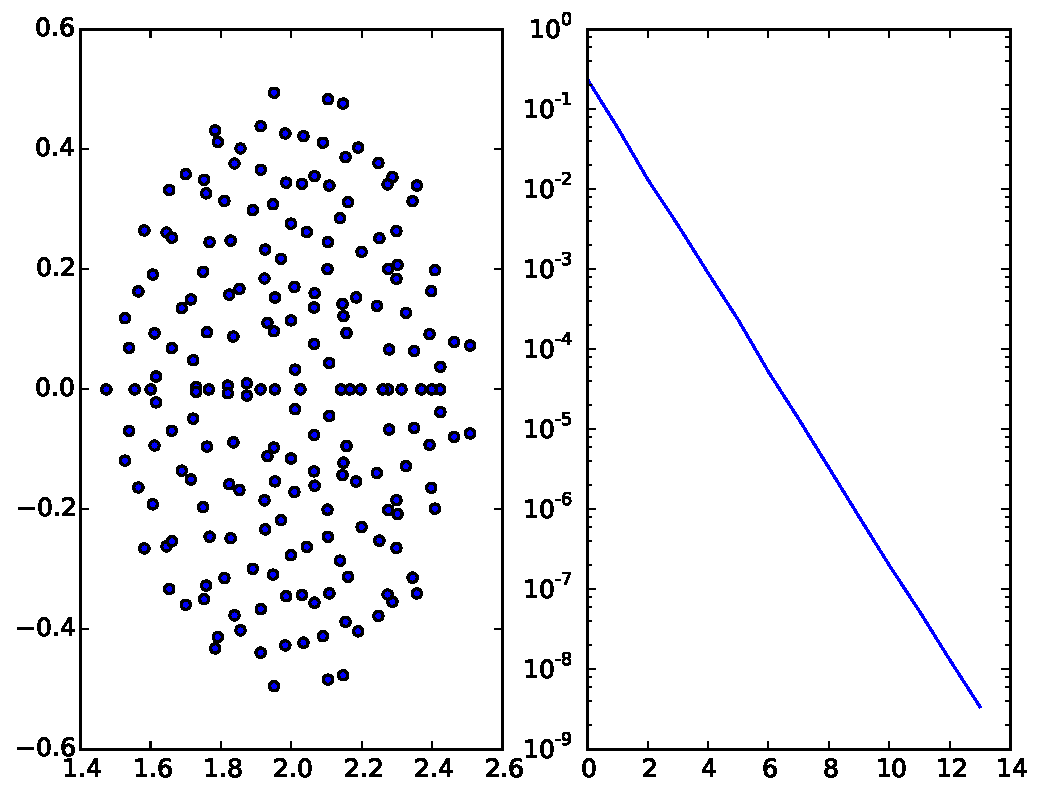
\includegraphics[width=.7\textwidth]{plot_gmres.pdf}
\caption{The left plot is the eigenvalues of the matrix $A_2$, which is defined in Problem \ref{prob:plot_gmres}.
The right plot is the convergence of the GMRES algorithm on $A_2$ with starting vector $\b = (1, 1, \ldots, 1)$.
This figure is one possible output of the function \li{plot_gmres()}.}
\label{fig:plot_gmres}
\end{figure}



\section*{Improving GMRES}
There are many ways to make the GMRES algorithm more robust and efficient.


\subsection*{Breakdowns in GMRES}
One of the selling points of GMRES is that it can't break down unless it reaches an exact solution.
In other words, the only way GMRES could break down is if a vector found by the Arnoldi iteration is 0.
That is, suppose, we have already computed 
\[\mathcal{K}_n(A, \b) = \text{span}\{\b, A\b, \ldots, A^{n-1}\b\} = \text{span}\{\q_1, \ldots, \q_n\}.\]
We next compute $A^n\b$ and orthogonalize it against $\mathcal{K}_n(A, \b)$, yielding $\q_{n+1}$.
But if $A^n\b \in \mathcal{K}_n(A,\b)$ then $\q_{n+1}$ will be 0, and our algorithm will break when we try to normalize $\q_{n+1}$.

In this situation, the least squares solution to \eqref{eq:GMRES_lstsq1} is an \emph{exact} solution to $A\x=\b$. 
In other words, $\b$ is in the $\text{span}\{\q_1, \ldots, \q_n\}$.  Fortunately, precautions against this have been taken in our implementation of the Arnoldi algorithm.

\begin{comment}
This problem is superfluous because we implemented our GMRES algorithm with the very Arnoldi algorithm referred to.

\begin{problem}
Update your solution to Problem \ref{prob:MyGMRES} to deal with the scenario described above.
Hint: Use something similar to lines 11-12 of the Arnoldi algorithm in Lab \ref{lab:kry_arnoldi}.
\label{prob:GMRES3}
\end{problem}
\end{comment}

% This section is poorly written. It is vague, not mathematically precise.
% If we ever want to include it, then it needs a lot of work.
\begin{comment}
\subsection*{Optimizing Least-Squares for GMRES (Optional)}
The Hessenberg structure and the Krylov subspace relations enable us to save time on the least-squares part of the problem if we use QR factorization.
Observe that if $H_n$ can be factored as $Q_n R_n$, where $Q_n$ is not the same matrix as above and $R_n$ is invertible upper triangular, we may solve the least squares problem by simply solving $R_n x_n=\norm{b} Q_{n}^{H}e_1$ via back substitution.
There are two ways in which we can speed up this process.
First, we take advantage of the Hessenberg structure by using the techniques from Problem \ref{prob:givens_hessenberg} in Lab \ref{lab:givens}.
Recall that the technique in this situation was to use Givens rotations to eliminate the subdiagonal elements one at a time.
This process, which was part of a previous lab, reduces the operation count from $O(n^3)$ to $O(n^2)$.
The second speedup comes from the fact that we already know the QR factorization for $H_{n-1}$ from the previous step of the algorithm.
This means that we can simply update the QR factorization from the previous step rather than computing it all over again.
Since $H_{n}$ has only one more column and row than $H_{n-1},$ all we need to do is update the last column by performing all previous Givens rotations on just the last column of $H_n$, which requires only $O(n)$ work.
Then we perform one final Givens rotation on $H_n$ to eliminate the new subdiagonal entry which was not present in $H_{n-1}$.
Thus, the QR factorization of $H_n$ can be reduced from an $O(n^3)$ process to only $O(n)$ using these special techniques.

The back substitution necessary to solve the least squares problem can also be reduced to an operation of $O(n)$.

The speedup from $O(n^3)$ to $O(n)$ is very good, but it can only partially alleviate the problems that come with a problem that is ill-suited for GMRES.
It may still be useful because it allows us to perform more iterations in a reasonable amount of time.
In many situations, the simple technique of the next section will keep $n$ low enough that the optimizations from this section are not critical.

 \begin{problem}
 \label{prob:GMRES2}
 (Optional) Modify MyGMRES to incorporate these optimizations, and call this program MyGMRES1.
 Run both programs on a series of five random $100\times 100$ matrices and compare the time each requires.
 Are the gains substantial?
 Try it again matrices of size $1000\times 1000$ or larger, and see how substantial the difference becomes.
 Try the same thing using the techniques of the next section.
 Explain why the difference in performance is less dramatic this time.
 \end{problem}
\end{comment}

\subsection*{GMRES with Restarts}
The first few iterations of GMRES have low spatial and temporal complexity. 
However, as $k$ increases, the $k^{th}$ iteration of GMRES becomes more expensive in both time and memory.
In fact, computing the $k^{th}$ iteration of GMRES for very large $k$ can be prohibitively complex.

This issue is addressed by using GMRES(k), or GMRES with restarts.
When $k$ becomes large, this algorithm restarts GMRES but with an improved initial guess.
GMRES with restarts is outlined in Algorithm \ref{alg:gmres_k}.


\begin{algorithm}
\begin{algorithmic}[1]
\Procedure{GMRES(k)}{$A, \b, \x_0, k, tol, restarts$}
  \State $n \gets 0$ \Comment{Initialize}
   \While{$n \leq restarts$}
	\State{ Perform the GMRES algorithm, obtaining a least squares solution $\y$}.
	\State{ If the desired tolerance was reached, return. Otherwise, continue.}
    \State $\x_0 \gets \y$
    \State $n \gets n + 1$
    \EndWhile
    \State \pseudoli{return} $\y, \,\, res$		\Comment{Return the approximate solution and the residual}
\EndProcedure
\end{algorithmic}
\caption{The GMRES(k) algorithm. This algorithm performs GMRES on a vector $\b$ and matrix $A$. It iterates $k$ times before restarting. 
It terminates after $restarts$ restarts or when the residual is less than $tol$, returning an approximate solution to $A\x=\b$ and the error in this approximation. }
\label{alg:gmres_k}
\end{algorithm}





The algorithm GMRES(k) will always have manageable spatial and temporal complexity, but it is less reliable than GMRES.
If the true solution $\x$ to $A\x=\b$ is nearly orthogonal to the Krylov subspaces $\mathcal{K}_n(A, \b)$ for $n\leq k$, then GMRES(k) could converge very slowly or not at all.

\begin{problem}
Implement Algorithm \ref{alg:gmres_k} with the following function.
\begin{lstlisting}
def gmres_k(A, b, x0, k=5, tol=1E-8, restarts=50):
    '''Use the GMRES(k) algorithm to approximate the solution to Ax=b.
    
    INPUTS:
    A        - A callable function that calculates Ax for any vector x.
    b        - A NumPy array.
    x0       - An arbitrary initial guess.
    k        - Maximum number of iterations of the GMRES algorithm before 
              restarting. Defaults to 5.
    tol      - Stop iterating if the residual is less than 'tol'. Defaults 
              to 1E-8.
    restarts - Maximum number of restarts. Defaults to 50.
    
    RETURN:
    Return (y, res) where 'y' is an approximate solution to Ax=b and 'res' 
    is the residual.
    '''
\end{lstlisting}

Compare the speed of \li{gmres()} from Problem \ref{prob:MyGMRES} and \li{gmres_k()} on the matrices in Problem \ref{prob:plot_gmres}.
\label{prob:GMRES3}
\end{problem}

\section*{GMRES in SciPy}
The GMRES algorithm is implemented in SciPy as the function \li{scipy.sparse.linalg.gmres()}.
Here we use this function to solve $A\x=\b$ where $A$ is a random $300 \times 300$ matrix and $\b$ is a random vector.

\begin{lstlisting}
>>> import numpy as np
>>> from scipy import sparse as spar
>>> from scipy import linalg as la
>>>
>>> A = np.random.rand(300, 300)
>>> b = np.random(300)
>>> x, info = spar.linalg.gmres(A, b)
>>> info
3000
\end{lstlisting}

The function outputs two objects: the approximate solution \li{x} and a constant \li{info} telling if the function converged.
If \li{info=0} then convergence occured; if \li{info} is positive then it equals the number of iterations performed.
In this case, the function performed 3000 iterations of GMRES before returning the approximate solution \li{x}.
We can check how close the solution is.
\begin{lstlisting}
>>> la.norm(A.dot(x)-b)
4.744196381683801
\end{lstlisting}

We can get a better approximation using GMRES with restarts. 
\begin{lstlisting}
>>> # Restart after 1000 iterations
>>> x, info = spar.linalg.gmres(A, b, restart=1000)
>>> info
0
>>> la.norm(A.dot(x)-b)
1.0280404494143551e-12
\end{lstlisting}
This time, the returned approximation \li{x} is about as close to a true solution as we could hope for.


